\documentclass[11pt]{article}

\usepackage[T1]{fontenc}
\usepackage[utf8]{inputenc}
\usepackage[margin=1in]{geometry}
\usepackage{amsmath}
\usepackage{booktabs}
\usepackage{tabularx}
\usepackage{longtable}
\usepackage{enumitem}
\usepackage{upquote}
\usepackage{xcolor}
\usepackage{tikz}
\usetikzlibrary{arrows.meta,positioning}
\usepackage{hyperref}

\newcolumntype{Y}{>{\raggedright\arraybackslash}X}

\title{Training Hide-and-Seek Agents with Graph-as-Policy:\\
How Our Program Uses Two Team Graphs and a Local LLM}
\author{}
\date{}

\begin{document}
\maketitle

%=====================================================================
\section{The Program in Brief}
%=====================================================================

\subsection{The idea}

Our first method trained a neural network with Proximal Policy Optimization
(PPO): the agents played millions of games, and learning slowly adjusted the
network's weights. Our new program, \texttt{train\_gap.py}, follows the
Graph-as-Policy (GaP) method of Chen et al.\ (arXiv:2607.05369) instead.

In GaP, the policy is not a neural network but a \textbf{graph}: a short,
readable plan built from simple skills, such as ``grab a box, take it to the
door, lock it''. A useful way to picture it is a team \emph{playbook}. Learning
means repeatedly rewriting the playbook and keeping only the versions that
actually win more games.

Following our professor's suggestion, there are \textbf{two graphs}: one for the
two hiders and one for the two seekers. They are improved in turns (hiders, then
seekers, then hiders again), so each team must keep adapting to the other.

\subsection{The game}

The environment is \textbf{exactly the same} as in our PPO run: the
hide-and-seek quadrant scenario with 2 hiders, 2 seekers, 2 lockable boxes, and
1 ramp that can be moved but not locked. A game (episode) lasts 80 steps: a
32-step \emph{preparation phase}, in which seekers are frozen and hiders can
prepare, followed by a 48-step \emph{play phase}. The quadrant has one or two
open doorways, controlled by $p_{\text{door}}$, as in our PPO run.

\subsection{What a team graph contains}

Each team graph says, for each of the team's two agents (its two
\emph{roles}):
\begin{itemize}
  \item what to do during \textbf{preparation}: a list of up to four
  \emph{segments}, done in order;
  \item what to do during \textbf{play}: a \emph{behaviour} (for example
  \texttt{search} or \texttt{chase}), optionally followed by more segments.
\end{itemize}
A \textbf{segment} is one small task of the form
\emph{grab an object} $\rightarrow$ \emph{take it somewhere} $\rightarrow$
\emph{lock it} $\rightarrow$ \emph{let go}. A segment can also have a
\textbf{gate}, a condition such as ``wait until all doors are sealed''. The graph
also has a few numeric \textbf{parameters}, such as movement speed, and a rule
for which agent gets which role. Section~\ref{sec:dictionary} defines every one
of these variables.

Two design choices keep the experiment fair:
\begin{itemize}
  \item \textbf{Only primitive skills.} There is no ``block the door'' or ``hide
  the ramp'' skill. To block a door, the graph must \emph{combine} grab a box,
  take it to the doorway, and lock it. So if such behaviour appears, it was
  discovered, not programmed.
  \item \textbf{Neutral start.} Both teams begin with a graph in which every agent
  just stands still. Every behaviour, including chasing, has to be found by
  training.
\end{itemize}

\subsection{How a graph plays a game}

During a game, a part of the program called the \textbf{graph executor} reads
each team's graph at every step and turns it into the same actions the PPO
agents used (move, turn, grab, lock). For each agent it:
(1) updates what the team knows, where opponents are seen only in the agent's
line of sight and are remembered after they disappear;
(2) runs the agent's current segment, moving on when it is finished, or skipping
it if it takes too long or is impossible;
(3) plans a path, through a doorway if needed, and moves the agent.
It also records whether each segment succeeded or failed, which is used later in
the report given to the LLM.

\subsection{How training works}

Training repeats the loop of Figure~\ref{fig:loop}. Each round improves
\emph{one} team's graph.

\begin{figure}[ht]
\centering
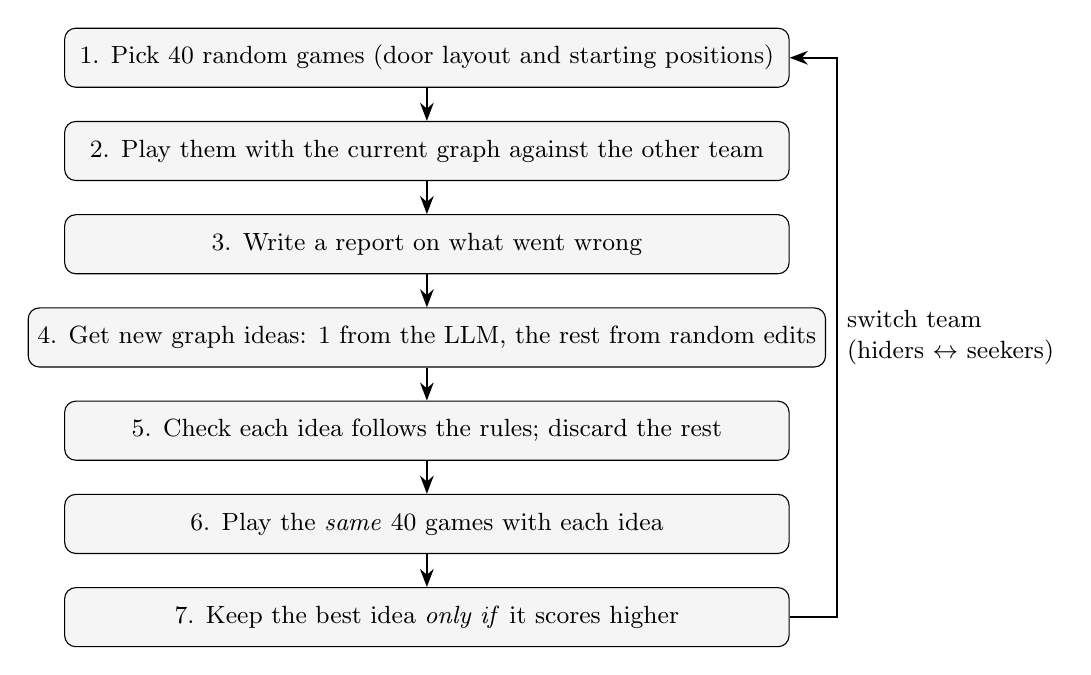
\begin{tikzpicture}[
  node distance=0.42cm,
  box/.style={draw, rounded corners, align=center, minimum width=9.2cm,
              minimum height=0.75cm, fill=gray!8, font=\small},
  arr/.style={-{Stealth[length=2.3mm]}, thick}]
  \node[box] (sample)  {1. Pick 40 random games (door layout and starting positions)};
  \node[box, below=of sample] (base) {2. Play them with the current graph against the other team};
  \node[box, below=of base] (fail) {3. Write a report on what went wrong};
  \node[box, below=of fail] (prop) {4. Get new graph ideas: 1 from the LLM, the rest from random edits};
  \node[box, below=of prop] (val)  {5. Check each idea follows the rules; discard the rest};
  \node[box, below=of val]  (reh)  {6. Play the \emph{same} 40 games with each idea};
  \node[box, below=of reh]  (acc)  {7. Keep the best idea \emph{only if} it scores higher};
  \draw[arr] (sample) -- (base);
  \draw[arr] (base) -- (fail);
  \draw[arr] (fail) -- (prop);
  \draw[arr] (prop) -- (val);
  \draw[arr] (val) -- (reh);
  \draw[arr] (reh) -- (acc);
  \draw[arr] (acc.east) -- ++(0.6,0) |- node[pos=0.25, right, align=left, font=\small]
        {switch team\\(hiders $\leftrightarrow$ seekers)} (sample.east);
\end{tikzpicture}
\caption{One round of training. The loop runs until 43.4 million games have been
played, the same budget as our PPO run.}
\label{fig:loop}
\end{figure}

Three details matter. First, in 30\% of the games the opponent is an
\emph{older} version of its graph, so a team cannot win only by exploiting the
newest opponent; this matches the opponent pool of our PPO run. Second, all ideas
are tested on the \emph{same} 40 games, so a better score reflects a better
graph, not luckier games. Third, the agents never ``think'' during a game: all
learning happens \emph{between} games, when graphs are rewritten.

\subsection{The role of the LLM}

The LLM (Qwen3~8B, running locally on our GPU through Ollama, free of charge) acts
as an \textbf{assistant coach}. Once per round, the program, not a person,
sends it a text message and receives one reply:

\begin{itemize}
  \item \textbf{What it reads:} fixed instructions (the allowed building blocks,
  the reply format, and the goal ``improve the objective''), the report on what
  went wrong, and the current graph. It never sees the game itself.
  \item \textbf{What we ordered it to do:} only rules and format. We never tell
  it a strategy such as ``block the doors''.
  \item \textbf{What it replies:} one new graph, written in JSON, with no
  explanation. It replies to the program, not to us.
  \item \textbf{Why it cannot cheat:} the program, not the LLM, decides. A reply
  that breaks the rules is discarded, and a valid one is kept only if it wins more
  games than the current graph.
\end{itemize}

This mirrors the GaP paper's key idea: the LLM \emph{proposes} changes, and
testing in simulation \emph{judges} them. The next section shows one complete,
real example.

%=====================================================================
\section{A Complete Real Example}
\label{sec:example}
%=====================================================================

This example is taken word for word from our 100{,}000-game pilot run, which
started from neutral graphs. It is round (iteration)~4, and it is the hiders'
turn to learn.

\subsection{The situation}

Both teams still had the neutral starting graph, in which every agent stands
still. The program had just played 40 games with it:

{\small
\begin{verbatim}
assign=fixed params={'gain': 4.0, 'damp': 0.5, 'tol': 0.3,
                     'offset': 0.15, 'seg_timeout': 30}
  role0 prep: (none) | play: stay
  role1 prep: (none) | play: stay
\end{verbatim}
}

The program then sent Qwen one request in two parts: a \textbf{system message}
containing the fixed orders, which is identical in every round, and a
\textbf{user message} containing this round's report.

\subsection{Part 1: The fixed orders (system message)}

The real message is a single paragraph. Below it is split into pieces, each
followed by what it means.

{\small
\begin{verbatim}
You are a robot skill-graph optimisation agent in a GaP harness.
\end{verbatim}
}
\noindent\textit{Meaning:} the LLM's job is to improve skill graphs.

{\small
\begin{verbatim}
Return exactly one JSON object. No Markdown, prose, or extra keys.
Boolean fields lock and release must be bare JSON booleans true or
false (not strings or numbers).
\end{verbatim}
}
\noindent\textit{Meaning:} reply with a graph only, no chat or explanation, in a
format the program can read.

{\small
\begin{verbatim}
Use this valid example for the required structure, then change values
only to improve the objective:
{"team": "hider", "assign": "fixed",
 "params": {"gain": 4.0, "damp": 0.5, "tol": 0.3, "offset": 0.15,
            "seg_timeout": 30},
 "roles": [
  {"prep": [{"acquire": null, "deliver": "wander", "lock": false,
             "release": false, "face": "target", "route": "door",
             "gate": null}],
   "play": {"behaviour": "stay", "target": "stay", "route": "door",
            "segments": []}},
  {"prep": [],
   "play": {"behaviour": "stay", "target": "stay", "route": "door",
            "segments": []}}]}
\end{verbatim}
}
\noindent\textit{Meaning:} an example of the \emph{shape} of a graph. It is
deliberately useless (one agent wanders, both stand still in play), so it gives
no strategy away.

{\small
\begin{verbatim}
Allowed values:
 assign in ['fixed', 'nearest_object'];
 segment.acquire in [None, 'box', 'ramp'];
 targets in ['door_block', 'door_inside', 'quadrant_interior',
   'quadrant_corner', 'ramp_inside', 'outside_wall', 'climb',
   'teammate', 'opponent', 'away_from_opponent', 'ramp', 'box',
   'wander', 'stay'];
 face in ['target', 'align', 'yaw0', 'yaw1', 'yaw2', 'yaw3'];
 route in ['door', 'direct'];
 play.behaviour in ['stay', 'flee', 'chase', 'search', 'go', 'segments'];
 params ranges {'gain': (1.0, 6.0), 'damp': (0.2, 0.8),
   'tol': (0.2, 0.6), 'offset': (0.0, 0.6), 'seg_timeout': (8, 40)};
 segment.gate in [None, 'teammate_inside', 'ramp_inside',
   'opponent_visible', 'doors_sealed', 'door'].
\end{verbatim}
}
\noindent\textit{Meaning:} the complete \textbf{vocabulary}. These are the only
words the LLM may use. Each is explained in Section~\ref{sec:dictionary}. The list
names building blocks but never says how to combine them.

{\small
\begin{verbatim}
Gate meanings: teammate_inside=other teammate entered quadrant,
ramp_inside=ramp is inside quadrant, opponent_visible=opponent
currently visible, doors_sealed=all doors blocked, door=one teammate
is near any doorway, null=no gate.
\end{verbatim}
}
\noindent\textit{Meaning:} what each ``wait until\ldots'' condition means.

{\small
\begin{verbatim}
Seekers cannot act in preparation.
Atomic skills only: compose them to improve the objective.
\end{verbatim}
}
\noindent\textit{Meaning:} one rule of the game, and the goal: combine the
building blocks to do better.

\subsection{Part 2: This round's report (user message)}

This part changes every round. The program wrote it after playing the 40 games.
Four of its eight failure lines are shown; the other four are similar.

{\small
\begin{verbatim}
# Rehearsal feedback - iteration 4 - learning team: hider

## Current graph
assign=fixed params={'gain': 4.0, 'damp': 0.5, 'tol': 0.3,
                     'offset': 0.15, 'seg_timeout': 30}
  role0 prep: (none) | play: stay
  role1 prep: (none) | play: stay

## Aggregate (n=40 instances)
- hider objective J (fraction of play steps all hiders hidden): 0.220
- hider win-rate: 0.23
- behaviour detection rates: {"chasing": 0.0, "door_blocking": 0.0,
  "ramp_use": 0.0, "ramp_defense": 0.0}
- mean first-seen play step: 33.0
- doors sealed+locked at prep end: 0.00,
  ramp inside quadrant at prep end: 0.15
- seekers entered quadrant: 0.00, mean max seeker z: 0.15

## Failure analysis (lost instances)
- p_door=0.25 doors=2 sealed=[False, False] ramp_inside=False
  boxes_moved=[0.0, 0.0] | seeker 2 saw hider 1 at play step 33
  (hider outside quadrant, seeker outside, seeker z=0.15)
  | segments: no segments executed
- p_door=0.75 doors=1 sealed=[False] ramp_inside=False
  boxes_moved=[0.0, 0.0] | seeker 2 saw hider 0 at play step 33
  (hider outside quadrant, seeker outside, seeker z=0.15)
  | segments: no segments executed
- p_door=1.00 doors=1 sealed=[False] ramp_inside=False
  boxes_moved=[0.0, 0.0] | seeker 2 saw hider 0 at play step 33
  (hider inside quadrant, seeker outside, seeker z=0.15)
  | segments: no segments executed
- p_door=0.25 doors=2 sealed=[False, False] ramp_inside=False
  boxes_moved=[0.0, 0.0] | hiders never seen
  | segments: no segments executed

## Current graph JSON
{"team": "hider", "assign": "fixed",
 "params": {"gain": 4.0, "damp": 0.5, "tol": 0.3, "offset": 0.15,
            "seg_timeout": 30},
 "roles": [{"prep": [], "play": {"behaviour": "stay", "target": "stay",
                                 "route": "door", "segments": []}},
           {"prep": [], "play": {"behaviour": "stay", "target": "stay",
                                 "route": "door", "segments": []}}]}

Return an improved graph for the hider team. Keep the team field
exactly 'hider'.
\end{verbatim}
}

\noindent In plain words, the report says: \emph{``Your hiders stood still.
They won only 23\% of games and were usually caught at the very first step of
the play phase. Nobody moved a box or sealed a door. Here is the current
playbook; give me a better one.''}

The request was sent with three settings: model \texttt{qwen3:8b},
temperature $0.3$, and JSON-only output (Section~\ref{sec:settings}).

\subsection{Part 3: Qwen's reply}

Qwen replied with a graph only, with no words. As printed in our training log:

{\small
\begin{verbatim}
assign=fixed params={'gain': 5.0, 'damp': 0.4, 'tol': 0.2,
                     'offset': 0.4, 'seg_timeout': 40.0}
  role0 prep: [when doors_sealed] grab ramp to ramp[align,direct] lock
        play: search
              then [when doors_sealed] grab ramp to ramp[align,direct] lock
  role1 prep: [when doors_sealed] grab box to box[align,direct] lock
        play: search
              then [when doors_sealed] grab box to box[align,direct] lock
\end{verbatim}
}

\noindent For example, the first agent's preparation segment, in JSON, is:

{\small
\begin{verbatim}
{"acquire": "ramp", "deliver": "ramp", "lock": true, "release": false,
 "face": "align", "route": "direct", "gate": "doors_sealed"}
\end{verbatim}
}

\noindent Read aloud: \emph{``When all doors are sealed, grab the ramp, carry it
straight to the ramp's own position while keeping it aligned, and lock it.''}
Compared with the old graph, Qwen made three changes: it added object-handling
segments, changed the play behaviour from \texttt{stay} to \texttt{search}, and
changed the parameters (faster, more precise, longer timeouts).

\subsection{Part 4: What the program did with the reply}

\paragraph{Rule check.} Every word in the reply is in the allowed vocabulary and
every field has the right type, so the reply passed. Many other replies in this
run failed this check; for example, a seeker graph that tried to \emph{grab} a
doorway was rejected with the message
\texttt{unknown segment acquire 'door\_block'}.

\paragraph{Playing the games.} The program played the same 40 games with the new
graph. Taken literally, the graph did this:
\begin{itemize}
  \item \textbf{Preparation:} every segment waits for \texttt{doors\_sealed},
  but nobody seals a door, so the condition never becomes true. The hiders wait,
  turning on the spot, and never grab anything.
  \item \textbf{Play:} the behaviour is \texttt{search}, so each hider patrols
  the points outside the doorways, the quadrant centre, and its corner, instead
  of standing still.
\end{itemize}

\paragraph{The decision.}

\begin{center}
\begin{tabular}{lcc}
  \toprule
  Same 40 games & Old graph (stand still) & Qwen's graph \\
  \midrule
  Hider objective $J$ & 0.220 & 0.542 \\
  Hider win rate      & 0.23  & 0.60  \\
  \bottomrule
\end{tabular}
\end{center}

\noindent The new graph scored clearly higher, so the program kept it and printed
\texttt{accepted LLM candidate for hider}. The old graph was stored as a ``past
opponent'', and in the next round the seekers had to adapt to the new hiders.

\subsection{What this example shows}

\begin{itemize}
  \item Part of Qwen's idea was \textbf{useful} (move during play instead of
  standing still) and part \textbf{did nothing}: a condition that never becomes
  true, a ramp carried to its own position, and an attempt to lock the ramp,
  which cannot be locked in our game. The improvement almost certainly came from
  the hiders moving, which partly took them into the quadrant.
  \item The program did not need Qwen's reasoning to be right. It kept the graph
  only because it \emph{measurably} won more games.
  \item This is exactly how GaP is meant to work: the LLM suggests, the
  simulation judges, and later rounds can remove useless parts or turn them into
  real strategies.
\end{itemize}

%=====================================================================
\section{Dictionary of All Variables}
\label{sec:dictionary}
%=====================================================================

Distances are in simulation units; the arena is $6 \times 6$ units. A ``step''
is one environment step; a game has 80 steps.

\subsection{Graph-level variables}

\begin{tabularx}{\linewidth}{@{}l l Y@{}}
  \toprule
  Variable & Values & Meaning \\
  \midrule
  \texttt{team}   & \texttt{hider}, \texttt{seeker} & Which team the graph controls. \\
  \texttt{assign} & \texttt{fixed} & Agent 1 of the team always plays role 0, agent 2 plays role 1. \\
                  & \texttt{nearest\_object} & At the start of each game, the roles are swapped if
                    that shortens the total distance from each agent to the first object its role must grab. \\
  \texttt{roles}  & exactly 2 & One plan per agent; each has \texttt{prep} and \texttt{play}. \\
  \texttt{prep}   & 0--4 segments & The plan for the preparation phase. Always empty for seekers, who are frozen. \\
  \texttt{play}   & a play node & What to do in the play phase (Section~\ref{sec:play}). \\
  \bottomrule
\end{tabularx}

\subsection{Parameters (\texttt{params})}

\begin{tabularx}{\linewidth}{@{}l l Y@{}}
  \toprule
  Parameter & Range & Meaning \\
  \midrule
  \texttt{gain}        & 1.0--6.0 & Speed: the desired speed is this number times the remaining distance
                                    to the goal, capped at 7 units/s. Higher means faster and more aggressive. \\
  \texttt{damp}        & 0.2--0.8 & How strongly the controller corrects the difference between the
                                    desired and actual velocity. Higher means snappier but possibly jerkier movement. \\
  \texttt{tol}         & 0.2--0.6 & Tolerance: how close (in units) something must get to its destination
                                    for a delivery to count as finished. \\
  \texttt{offset}      & 0.0--0.6 & Placement fine-tuning: how far inside a doorway a box is placed for
                                    \texttt{door\_block}, and how much extra space is left from the wall for
                                    \texttt{outside\_wall}. \\
  \texttt{seg\_timeout} & 8--40 steps & Maximum time for one segment. When it runs out, the segment is
                                    skipped (recorded as \texttt{timeout}). Doubled for \texttt{climb}. \\
  \bottomrule
\end{tabularx}

\subsection{The play node}
\label{sec:play}

\begin{tabularx}{\linewidth}{@{}l Y@{}}
  \toprule
  Field / value & Meaning \\
  \midrule
  \texttt{behaviour} & What the agent does in the play phase: \\
  \quad\texttt{stay}     & Stand still. \\
  \quad\texttt{flee}     & Move 1.5 units away from the nearest opponent seen; if none has been seen,
                           stand and turn to look around. \\
  \quad\texttt{chase}    & Move to where an opponent was last seen; if none has been seen, \texttt{search}. \\
  \quad\texttt{search}   & Patrol in a loop: a point outside each doorway, the quadrant centre, and the
                           quadrant corner. \\
  \quad\texttt{go}       & Go to the play \texttt{target} using the play \texttt{route}. \\
  \quad\texttt{segments} & Run the play segments in order, then go to the play \texttt{target}. \\
  \texttt{target}    & Destination used by \texttt{go} and after \texttt{segments} (one of the targets in
                       Section~\ref{sec:targets}). \\
  \texttt{route}     & \texttt{door} or \texttt{direct} (see segment \texttt{route} below). \\
  \texttt{segments}  & 0--4 segments run during play, only if \texttt{behaviour} is \texttt{segments}. \\
  \bottomrule
\end{tabularx}

\subsection{Segment fields}

\begin{tabularx}{\linewidth}{@{}l l Y@{}}
  \toprule
  Field & Values & Meaning \\
  \midrule
  \texttt{acquire} & \texttt{null} & Do not grab anything; just go to \texttt{deliver}. \\
                   & \texttt{box}  & Go to the nearest free, unlocked box and grab it. \\
                   & \texttt{ramp} & Go to the ramp and grab it. \\
  \texttt{deliver} & a target & Where to take the object, or where to go if nothing is carried
                                (Section~\ref{sec:targets}); \texttt{null} means no movement. \\
  \texttt{lock}    & \texttt{true}/\texttt{false} & At the destination, lock the carried box. Locked
                     boxes cannot be moved by the other team. The ramp cannot be locked. \\
  \texttt{release} & \texttt{true}/\texttt{false} & Let go of the object at the end; if \texttt{false},
                     keep holding it. \\
  \texttt{face}    & \texttt{target} & While moving, face the destination. \\
                   & \texttt{align}  & Rotate a carried ramp so its slope rises towards the nearest
                                       quadrant wall, so it can be climbed. \\
                   & \texttt{yaw0}--\texttt{yaw3} & Turn to a fixed direction: 0\textdegree,
                                       90\textdegree, 180\textdegree, or 270\textdegree. \\
  \texttt{route}   & \texttt{door}   & If the destination is on the other side of the quadrant wall, go
                                       through an open doorway; also walk around the quadrant instead of
                                       into its wall. \\
                   & \texttt{direct} & Go in a straight line. \\
  \texttt{gate}    & \texttt{null}   & Start immediately. \\
                   & \texttt{teammate\_inside}  & Wait until the teammate is inside the quadrant. \\
                   & \texttt{ramp\_inside}      & Wait until the ramp is inside the quadrant. \\
                   & \texttt{opponent\_visible} & Wait until a teammate can see an opponent. \\
                   & \texttt{doors\_sealed}     & Wait until every doorway is blocked by a box. \\
                   & \texttt{door}              & Wait until a teammate is near a doorway. \\
  \bottomrule
\end{tabularx}

\medskip
While waiting at a gate, the agent stands still and turns to look around (and
keeps holding an object if it has one). A segment is \emph{skipped} if there is no
suitable object or target, or when \texttt{seg\_timeout} runs out.

\subsection{Targets (places to go)}
\label{sec:targets}

\begin{tabularx}{\linewidth}{@{}l Y@{}}
  \toprule
  Target & Meaning \\
  \midrule
  \texttt{door\_block}         & A point in the nearest doorway that is not already sealed or claimed
                                 by the teammate, moved \texttt{offset} units inwards. Taking a box here
                                 and locking it seals the door. \\
  \texttt{door\_inside}        & A point just inside that doorway (0.95 units in). \\
  \texttt{quadrant\_interior}  & The centre of the quadrant. \\
  \texttt{quadrant\_corner}    & The far corner of the quadrant, the point furthest from the doorways. \\
  \texttt{ramp\_inside}        & Same point as \texttt{quadrant\_corner}; the name suggests storing the
                                 ramp there. \\
  \texttt{outside\_wall}       & A point just outside the nearest quadrant wall where a ramp sits flush
                                 against it, plus \texttt{offset}. \\
  \texttt{climb}               & The quadrant centre, approached in a straight line; with a ramp against
                                 the wall, this takes a seeker up and over it. \\
  \texttt{teammate}            & The teammate's current position. \\
  \texttt{opponent}            & Where the nearest opponent was last seen. \\
  \texttt{away\_from\_opponent} & 1.5 units directly away from the nearest opponent seen; it stays
                                 inside the quadrant if the agent is already inside. \\
  \texttt{ramp}, \texttt{box}  & The ramp's position, or the nearest box's position. \\
  \texttt{wander}              & A random point in the arena, replaced by a new one when reached. \\
  \texttt{stay}                & The agent's current position. \\
  \bottomrule
\end{tabularx}

\subsection{Variables in the feedback report}

\begin{tabularx}{\linewidth}{@{}l Y@{}}
  \toprule
  Report item & Meaning \\
  \midrule
  \texttt{iteration}, learning team & The round number and the team being improved. \\
  \texttt{n} instances & The number of games played (40); a game is dropped if the physics engine
                         becomes unstable. \\
  hider objective \texttt{J} & The fraction of play steps in which \emph{both} hiders were hidden,
                         averaged over the games. 1 is perfect hiding; 0 means always seen. \\
  hider win-rate & The fraction of games the hiders won ($J > 0.5$ in that game). \\
  behaviour detection rates & How often each of the four emergent behaviours was detected
                         (Section~\ref{sec:detectors}). \\
  mean first-seen play step & The step (1--80) at which a seeker first saw a hider, averaged over
                         games. Play starts after step 32, so 33 means caught immediately. \\
  doors sealed+locked at prep end & The fraction of open doorways blocked by a locked box when
                         preparation ended. \\
  ramp inside quadrant at prep end & The fraction of games in which the ramp was inside the quadrant
                         when preparation ended. \\
  seekers entered quadrant & The fraction of games in which a seeker got inside the quadrant. \\
  mean max seeker \texttt{z} & The average highest height a seeker reached. Standing on the floor is
                         about 0.15; clearly higher means it climbed something. \\
  \midrule
  \texttt{p\_door} & The door setting of that game: the probability that one of the two doorways is
                         walled off. \\
  \texttt{doors} & The number of open doorways in that game (1 or 2). \\
  \texttt{sealed} & For each open doorway, whether a locked box was blocking it. \\
  \texttt{ramp\_inside} & Whether the ramp ended preparation inside the quadrant. \\
  \texttt{boxes\_moved} & How far each box was moved during preparation, in units. \\
  seeker $i$ saw hider $j$ & Who was caught first, and when. Agents 0 and 1 are hiders; agents 2
                         and 3 are seekers. Also reports whether each was inside the quadrant and the
                         seeker's height. \\
  \texttt{segments} & What happened to each segment, written as \texttt{prep0/1:done@12}: phase
                         (\texttt{prep} or \texttt{play}), role (0 or 1), segment number, outcome, and the
                         step. Outcomes: \texttt{done}; \texttt{timeout}; \texttt{dropped} (lost grip of
                         the object); \texttt{no\_target} (no valid destination, for example all doors
                         already sealed); \texttt{no\_object} (nothing suitable to grab). \\
  \bottomrule
\end{tabularx}

\subsection{Settings sent with each request}
\label{sec:settings}

\begin{tabularx}{\linewidth}{@{}l l Y@{}}
  \toprule
  Setting & Value & Meaning \\
  \midrule
  model           & \texttt{qwen3:8b} & The local language model (8 billion parameters), run by Ollama. \\
  temperature     & 0.3 & How random the replies are. 0 always gives the same answer; higher gives more
                          varied ideas. 0.3 is fairly consistent. \\
  response format & JSON object & Asks the model to reply in machine-readable JSON only. \\
  \bottomrule
\end{tabularx}

%=====================================================================
\section{Scoring and Behaviour Detection}
%=====================================================================

\subsection{Score}

The score uses the same zero-sum reward as the environment. In each game,
\[
  J = \frac{\text{play steps in which all hiders are hidden}}{\text{48 play steps}}.
\]
Hiders try to maximise $J$ and seekers try to maximise $1-J$. A new graph is kept
only if its score on the same 40 games beats the current graph's score by more
than $0.01$; a tiny penalty per segment favours simpler graphs. The hiders' mean
episode reward shown in our plot is $(2J-1)\times 48$, and the seekers' is its
negative.

\subsection{Emergent-behaviour detectors}
\label{sec:detectors}

After every game, the program checks the simulation for the four behaviours we
studied with PPO:

\begin{tabularx}{\linewidth}{@{}l Y@{}}
  \toprule
  Behaviour & Detected when \\
  \midrule
  Chasing            & A moving seeker within 3 units of a hider heads towards it during most of
                       the steps in which it is pursuing. \\
  Door blocking      & At the end of preparation, every open doorway is sealed by a locked box. \\
  Seeker ramp use    & A seeker enters the quadrant over the wall, not through a doorway, while
                       elevated. \\
  Hider ramp defense & The ramp started outside the quadrant and the hiders moved it inside during
                       preparation. \\
  \bottomrule
\end{tabularx}

\medskip
A behaviour's \emph{onset} is recorded the first time it is detected in at least
30\% (chasing, ramp use) or 50\% (door blocking, ramp defense) of a round's games.

%=====================================================================
\section{Budget and Outputs}
%=====================================================================

The full run uses the same budget as our PPO run: \textbf{43.4 million games}.
Each round plays up to $40 + 6 \times 40 = 280$ games, using 14 parallel
simulations. Unlike PPO, there are no \texttt{.npz} weight files: a policy is just
a small JSON graph. After every round the program saves:
\begin{itemize}
  \item \texttt{best\_hider\_graph.json}, \texttt{best\_seeker\_graph.json}: the
  current graphs, which can be rendered to video;
  \item \texttt{gap\_state.json}: everything needed to resume after a restart;
  \item \texttt{learning\_curve.png} and \texttt{history.csv}: rewards, win rate,
  and the four behaviour rates over training;
  \item \texttt{feedback/}: every report sent to the LLM.
\end{itemize}

%=====================================================================
\section{Differences from the GaP Paper}
%=====================================================================

Our program is an \textbf{adaptation} of GaP, not an exact reproduction:
\begin{itemize}
  \item \textbf{Task:} the paper improves one robot's graph for repeated
  manipulation tasks; we improve two competing team graphs whose opponent keeps
  changing.
  \item \textbf{Model:} the paper used Gemini~3.1 Flash-Lite; we use Qwen3~8B
  locally.
  \item \textbf{Agents:} the paper uses an orchestrator and several specialised
  LLM agents; we use one graph-update request per round.
  \item \textbf{Search:} we add random structural edits alongside the LLM, so
  that learning continues when the LLM's reply is invalid or unhelpful.
  \item \textbf{Simulator and skills:} the paper uses Isaac Sim and robot skills;
  we use the MuJoCo hide-and-seek environment and our own primitive skills.
\end{itemize}

\end{document}
